\documentclass{beamer}
\usepackage[portuguese]{babel}
\usepackage[utf8]{inputenc}
\usetheme{metropolis}

\title{Sistema de Mercado em Assembly 32bits}
\author{Gustavo Henrique Trassi Ganaza \and Yoshiyuki Fugie}
\date{\today}

\begin{document}

\begin{frame}
    \titlepage
\end{frame}

\begin{frame}{Arquitetura do Sistema de Gerenciamento de Supermercado}
    \begin{itemize}
        \item Sistema implementado em Assembly x86 32 bits
        \item Baseado em lista ligada para armazenamento de produtos
        \item Funcionalidades: CRUD, consultas financeiras, relatórios e persistência em disco
    \end{itemize}
\end{frame}

\begin{frame}{Arquivos e Estruturas}
    \begin{itemize}
        \item \textbf{Arquivo principal:} supermercado.s (Assembly)
        \item \textbf{Armazenamento:} produtos.bin (binário)
        \item \textbf{Relatórios:} relatorio.txt (texto)
        \item \textbf{Instruções para compilação:} makefile
        \begin{itemize}
            \item Compila com \texttt{gcc -m32}, portanto é necessário ter o pacote  \texttt{gcc-multilib} instalado.
        \end{itemize}
    \end{itemize}
\end{frame}

\begin{frame}{Armazenamento em Arquivo Binário}
    \begin{itemize}
        \item \textbf{Arquivo:} produtos.bin (modo binário)
        \item \textbf{Processo de gravação (save\_list):}
        \begin{itemize}
            \item Abre arquivo com fopen em modo escrita ("wb")
            \item Para cada nó:
            \begin{itemize}
                \item Copia 148 bytes de dados (excluindo ponteiro) para um buffer
                \item Escreve buffer no arquivo com fwrite
            \end{itemize}
            \item Fecha arquivo com fclose
        \end{itemize}
        \item \textbf{Processo de leitura (load\_list):}
        \begin{itemize}
            \item Abre arquivo em modo leitura ("rb")
            \item Lê blocos de 148 bytes (cada corresponde a um produto)
            \item Para cada bloco: aloca memória, copia dados, insere na lista
        \end{itemize}
    \end{itemize}
\end{frame}

\begin{frame}[fragile]{Alocação de Espaço para Produtos}
    \begin{itemize}
        \item Cada produto é um nó na lista ligada
        \item Tamanho total: 152 bytes (produto\_size)
        \item Estrutura do nó:
    \end{itemize}
    \begin{verbatim}
; Offsets (em bytes):
;   0: Ponteiro para próximo nó (4 bytes)
;   4: Nome (50 bytes)
;  54: Lote (20 bytes)
;  74: Tipo (4 bytes - índice para tabela de tipos)
;  78: Dia/Mês/Ano (4 bytes cada)
;  90: Fornecedor (50 bytes)
; 140: Quantidade (4 bytes)
; 144: Preço de compra (4 bytes - centavos)
; 148: Preço de venda (4 bytes - centavos)
    \end{verbatim}
\end{frame}

\begin{frame}{Menu de Operações}
    \begin{figure}
        \centering
        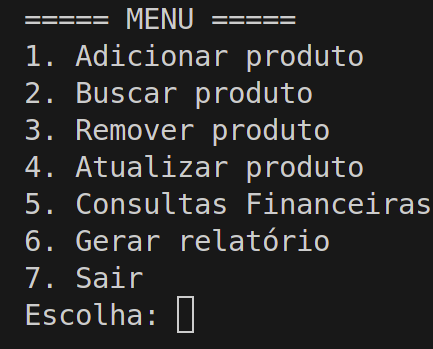
\includegraphics[width=0.7\textwidth]{img/menu-inicial.png}
    \end{figure}
\end{frame}

\begin{frame}{Função add\_product\_interactive}
    \textbf{Fluxo interativo via terminal:}
    \begin{enumerate}
        \item Aloca memória com malloc(152)
        \item Lê campos do usuário:
        \begin{itemize}
            \item read\_string\_with\_prompt para strings (nome, lote, fornecedor)
            \item scanf para números (tipo, datas, quantidades, preços)
        \end{itemize}
        \item Insere nó na lista com insert\_sorted (ordem alfabética por nome)
    \end{enumerate}
\end{frame}

\begin{frame}{Exemplo add\_product\_interactive}
    \begin{figure}
        \centering
        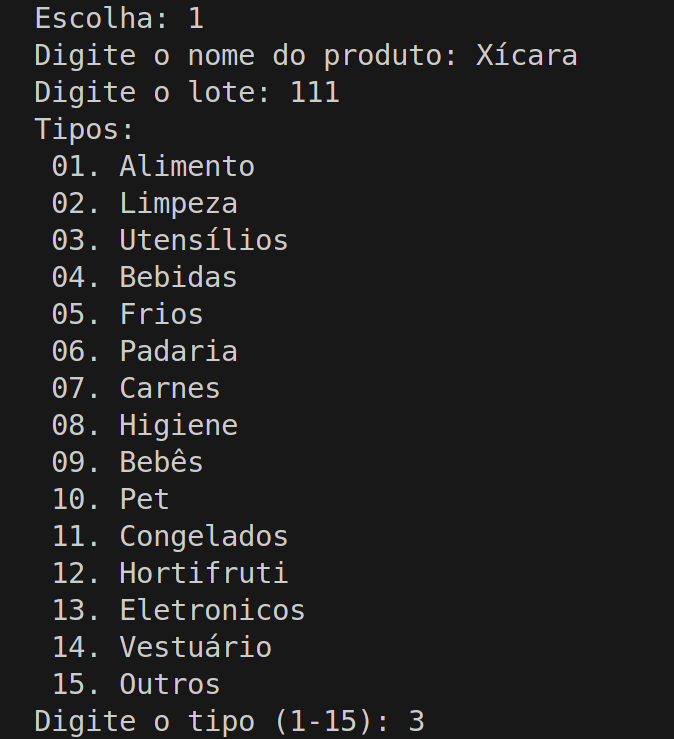
\includegraphics[width=0.6\textwidth]{img/add-1.png}
    \end{figure}
\end{frame}

\begin{frame}{Exemplo add\_product\_interactive}
    \begin{figure}
        \centering
        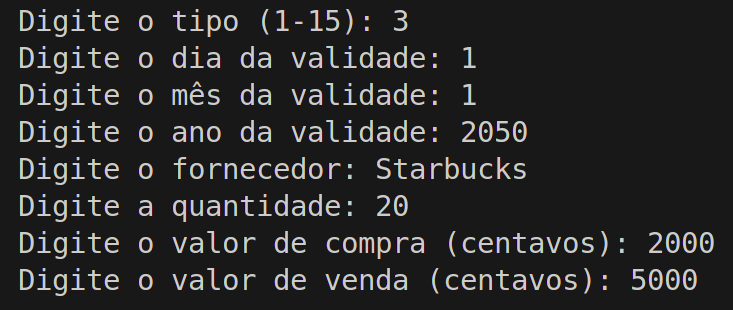
\includegraphics[width=0.6\textwidth]{img/add-2.png}
    \end{figure}
\end{frame}

\begin{frame}{Função search\_product}
    \begin{itemize}
        \item \textbf{Entrada:} Nome do produto (via str\_busca\_prompt)
        \item \textbf{Algoritmo:}
        \begin{itemize}
            \item Percorre a lista ligada
            \item Para cada nó:
            \begin{itemize}
                \item Compara nome com strcmp
                \item Se igual, imprime detalhes com print\_product
            \end{itemize}
        \end{itemize}
        \item \textbf{Saída:} Todos os produtos com nomes correspondentes
    \end{itemize}
\end{frame}

\begin{frame}{Função search\_product}
    \begin{figure}
        \centering
        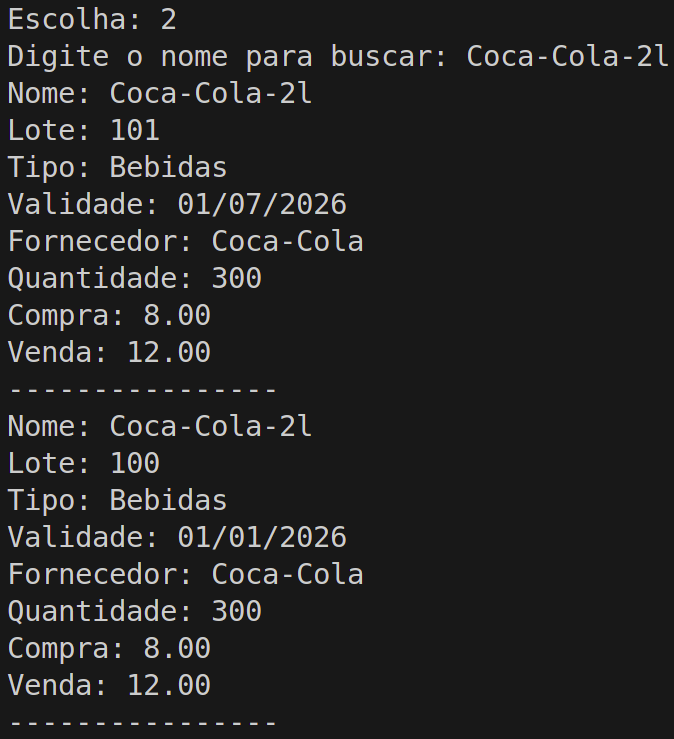
\includegraphics[width=0.6\textwidth]{img/busca.png}
    \end{figure}
\end{frame}

\begin{frame}{Função remove\_product\_interactive}
    \begin{itemize}
        \item \textbf{Entrada:} Nome + lote do produto
        \item \textbf{Passos:}
        \begin{enumerate}
            \item Busca nó na lista (compara nome e lote)
            \item Ajusta ponteiros:
            \begin{itemize}
                \item Se nó anterior existe: anterior-\textgreater next = atual-\textgreater next
                \item Se é o primeiro: head = atual-\textgreater next
            \end{itemize}
            \item Libera memória com free(atual)
        \end{enumerate}
        \item \textbf{Mensagens:} "Produto removido" ou "não encontrado"
    \end{itemize}
\end{frame}

\begin{frame}{Exemplo remove\_product\_interactive}
    \begin{figure}
        \centering
        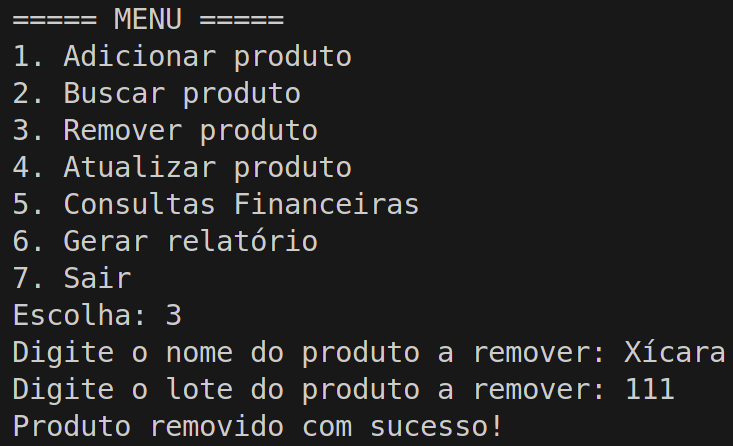
\includegraphics[width=0.6\textwidth]{img/remover.png}
    \end{figure}
\end{frame}

\begin{frame}{Função update\_product\_interactive}
    \begin{itemize}
        \item \textbf{Entrada:} Nome + lote do produto
        \item \textbf{Fluxo:}
        \begin{enumerate}
            \item Busca nó na lista
            \item Pergunta campo a atualizar (quantidade ou preço de venda)
            \item Lê novo valor e atualiza o campo no nó
        \end{enumerate}
        \item \textbf{Campos atualizáveis:}
        \begin{itemize}
            \item Quantidade (offset 140)
            \item Preço de venda (offset 148)
        \end{itemize}
    \end{itemize}
\end{frame}

\begin{frame}{Exemplo update\_product\_interactive}
    \begin{figure}
        \centering
        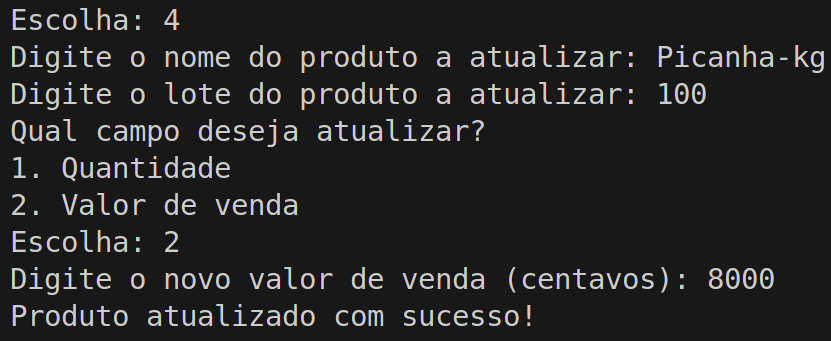
\includegraphics[width=0.8\textwidth]{img/update.png}
    \end{figure}
\end{frame}

\begin{frame}{Consultas Financeiras}
    \textbf{Opções:}
    \begin{itemize}
        \item \textbf{Total de compra:} Soma quantidade x preço\_compra (via total\_compra)
        \item \textbf{Total de venda:} Soma quantidade x preço\_venda (via total\_venda)
        \item \textbf{Lucro total:} total\_venda - total\_compra (via lucro\_total)
        \item \textbf{Capital perdido:} Soma de produtos vencidos (compara datas via capital\_perdido)
    \end{itemize}
    \vspace{0.5cm}
    \textbf{Formatação:} Valores em reais/centavos (ex: printf("\%d.\%02d"))
\end{frame}

\begin{frame}{Submenu de Consultas}
    \begin{figure}
        \centering
        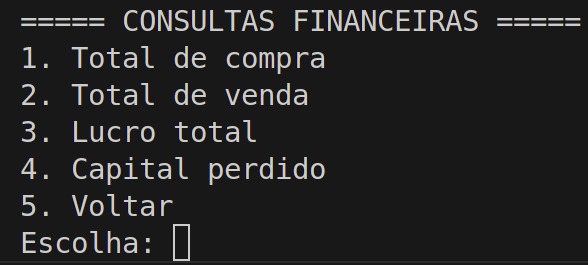
\includegraphics[width=0.7\textwidth]{img/consulta-1.png}
    \end{figure}
\end{frame}

\begin{frame}{Função total\_compra, total\_venda e lucro\_total}
    \textbf{Total compra}
    \begin{itemize}
        \item \textbf{Entrada:} Lista de produtos
        \item \textbf{Processo:}
        \begin{enumerate}
            \item Percorre a lista ligada
            \item Para cada nó:
            \begin{itemize}
                \item Multiplica quantidade pelo preço de compra/venda
                \item Acumula o total
            \end{itemize}
        \end{enumerate}
    \end{itemize}

    \textbf{Total venda}
    \begin{itemize}
        \item Similar ao total\_compra, mas usa preço de venda
    \end{itemize}


    \textbf{Lucro Total:} chama total\_venda e total\_compra, e faz a subtração
\end{frame}

\begin{frame}{Função capital\_perdido}
    \textbf{capital\_perdido}:
    \begin{enumerate}
        \item Pede a data atual ao usuário.
        \item Para cada produto, compara a data de validade com a data atual usando \texttt{compare\_dates}.
        \item Se a validade for anterior à data atual, soma \texttt{quantidade * valor\_compra} ao total perdido.
    \end{enumerate}
\end{frame}

\begin{frame}{Exemplo total\_compra}
    \begin{figure}
        \centering
        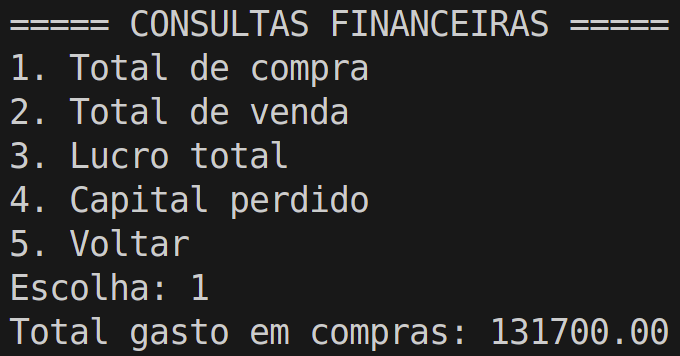
\includegraphics[width=0.6\textwidth]{img/total-compra.png}
    \end{figure}   
\end{frame}

\begin{frame}{Exemplo total\_venda}
    \begin{figure}
        \centering
        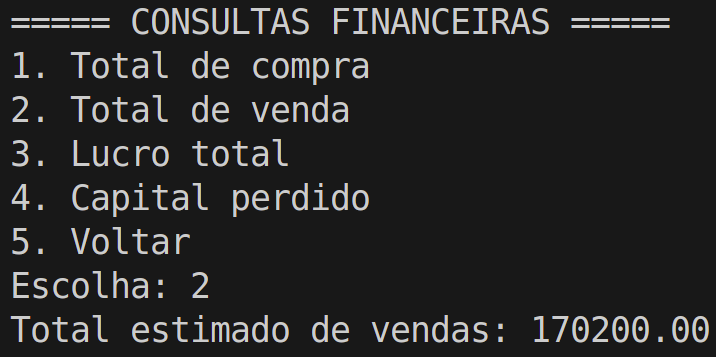
\includegraphics[width=0.6\textwidth]{img/total-venda.png}
    \end{figure}
\end{frame}

\begin{frame}{Exemplo lucro\_total}
    \begin{figure}
        \centering
        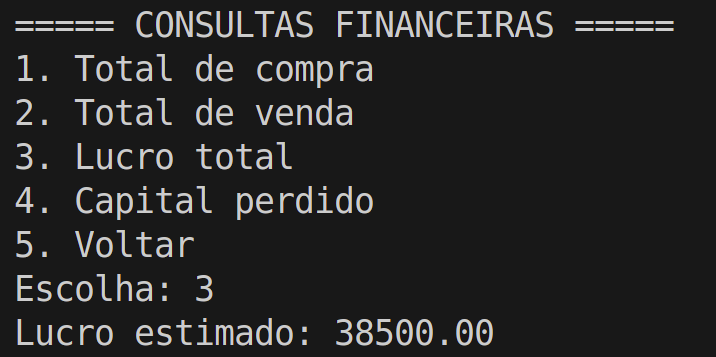
\includegraphics[width=0.6\textwidth]{img/lucro.png}
    \end{figure}   
\end{frame}

\begin{frame}{Exemplo capital\_perdido}
    \begin{figure}
        \centering
        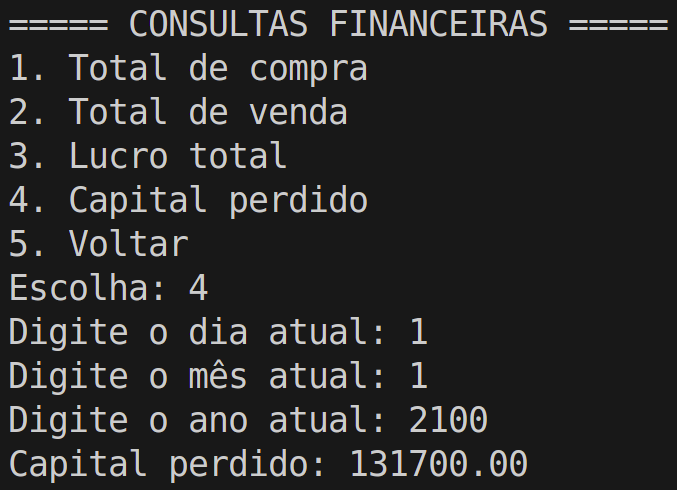
\includegraphics[width=0.6\textwidth]{img/capital-perdido.png}
    \end{figure}   
\end{frame}


\begin{frame}{Função generate\_report}
    \begin{itemize}
        \item \textbf{Arquivo de saída:} relatorio.txt (modo texto)
        \item \textbf{Ordenação opcional:}
        \begin{itemize}
            \item Por nome (padrão)
            \item Por quantidade (crescente, via sort\_by\_quantity)
            \item Por validade (mais antiga primeiro, via sort\_by\_date)
        \end{itemize}
        \item \textbf{Técnica:}
        \begin{enumerate}
            \item Converte lista em array de ponteiros
            \item Ordena array com bubble sort
            \item Grava produtos no arquivo com print\_product\_to\_file (usa fprintf)
        \end{enumerate}
    \end{itemize}
\end{frame}

\begin{frame}{Submenu de Relatórios}
    \begin{figure}
        \centering
        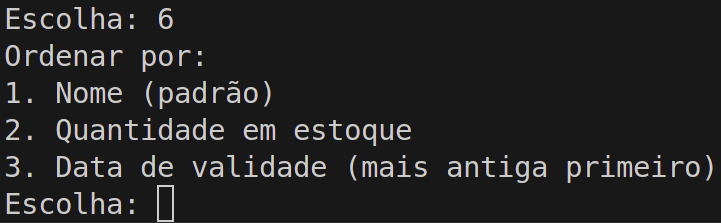
\includegraphics[width=0.8\textwidth]{img/submenu-relatorio.png}
    \end{figure}
\end{frame}

\begin{frame}{Exemplo generate\_report}
    \begin{figure}
        \centering
        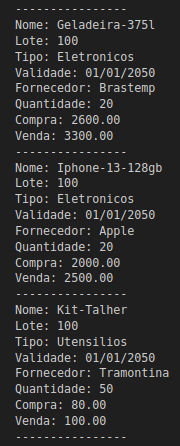
\includegraphics[width=0.3\textwidth]{img/relatorio-nome.png}
    \end{figure}
\end{frame}

\begin{frame}{Exemplo generate\_report (Ordenação por Quantidade)}
    \begin{figure}
        \centering
        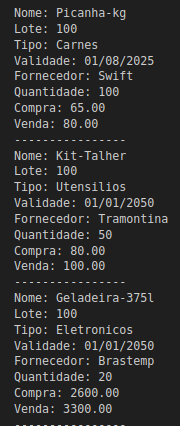
\includegraphics[width=0.3\textwidth]{img/relatorio-quantidade.png}
    \end{figure}
\end{frame}

\begin{frame}{Exemplo generate\_report (Ordenação por Validade)}
    \begin{figure}
        \centering
        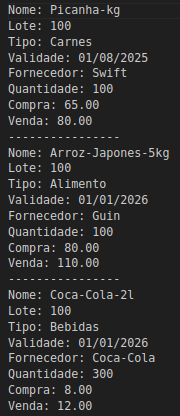
\includegraphics[width=0.3\textwidth]{img/relatorio-validade.png}
    \end{figure}
\end{frame}

\begin{frame}[plain]
\end{frame}

\end{document}